\chapter{提案手法}

本章では提案する手法の詳細について説明する.

\section{提案手法の概要}
\begin{figure}[h]
  \begin{center}
    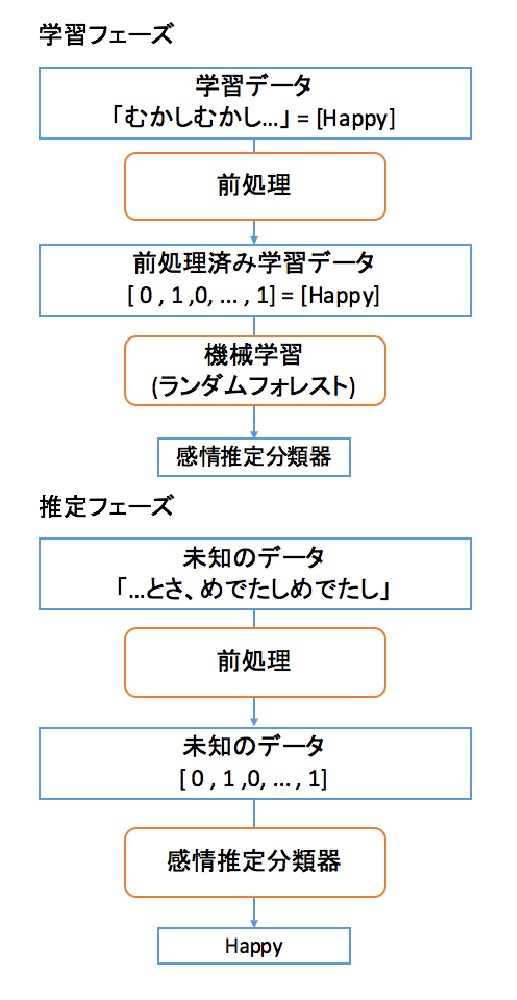
\includegraphics[clip,width=7.0cm]{fig/method-2.eps}
    \caption{提案手法の概要}
    \label{fig:method}
  \end{center}
\end{figure}

提案手法の概要を図\ref{fig:method}に示す.
本手法では,物語中のすべての文に対し文中に含まれる単語の出現を手がかりに朗読に最も適切もしくは自然と感じる感情を推定する.
感情のクラスはNormal,Happy,Sad,Angryの4種類とした.
まず,学習データとして各文に,それぞれ適切と思われる感情を人手で割り当てたものを用意する.
これに対し前処理を行いランダムフォレストを用いて学習を行う.
そして未知の入力文が与えられた場合に,感情クラスの1つを自動的に推定する他クラス分類を行うのが本手法である.

\subsection{機能語のみによる推定}
本手法は,学習と推定の際に文から内容語(名詞,動詞,形容詞,形容動詞)を取り除き,機能語のみで推定を行う.
なぜならば,未知の物語の感情を推定を目的としているため,学習データが特定の物語に依存していては推定精度が低くとなると考えられるからである.
例えば「鬼」がネガティブに描かれている物語を学習データとして,別の「鬼」がポジティブに描かている物語を推定した場合にネガティブな感情に推定されてしまう恐れがある.
一方,機能後は「しまう」や「ところが」など,朗読時の抑揚などに関係すると考えられる重要な助詞やや接続詞を含む.
したがって,内容語を排除し排除し,機能語のみで推定を行う.

\subsection{前処理}
\begin{figure}[h]
  \begin{center}
    \includegraphics[clip,width=7.0cm]{fig/method.eps}
    \caption{前処理の手順}
    \label{fig:pre}
  \end{center}
\end{figure}

前処理の概要を図\ref{fig:pre}に示す.
まず,物語の文章を文に分ける際は,基本的に句点で区切る.
カギ括弧で囲まれているセリフ部分はカギ括弧で区切り,カギ括弧内のセリフについても句点で区切る.
次に,形態素解析を行い単語ごとに分割しそれぞれの単語を基本形に変換する.
そして,形態素解析の結果から内容語を削除し機能語のみにする.
最後に,文中に単語が含まれるか否かを示すベクトル(Bag-of-words)に変換する.

\subsection{分類器の生成}
一般に,入力データに対して,予め定義された複数のクラスから一つを推定する手法としては機械学習の教師あり学習が適応できる.
本研究では,その1つであるランダムフォレストを用いて推定を行う.
ランダムフォレストは複数の決定木を用いて識別などを行うアンサンブル学習アルゴリズムである.
また,精度を向上させるために,正確度を指標としてグリットサーチを用いて最適なパラメタを探索する.
%TODO
%本研究で調整したパラメタはの\ref{parameter}通りである.
